%\documentclass[aspectratio=169]{beamer}
\documentclass[t]{beamer}

\usepackage{./beamer-itmo/beamer-itmo}

\usepackage{graphicx} % support of images
\usepackage{wrapfig} % support of wrapping figures by text
%\usepackage{float} % let you insert images where you really want
\usepackage{mathtext}
\usepackage{braket}
\usepackage{amsmath,amsfonts,amssymb,amsthm,mathtools}
\usepackage{mathrsfs}
\usepackage{icomma}
\usepackage{subcaption}

\usepackage{media9}

\uselanguage{russian}
\languagepath{russian}
\deftranslation[to=russian]{Theorem}{Теорема}
\deftranslation[to=russian]{Definition}{Определение}
\deftranslation[to=russian]{Definitions}{Определения}
\deftranslation[to=russian]{Corollary}{Следствие}
\deftranslation[to=russian]{Fact}{Факт}
\deftranslation[to=russian]{Example}{Пример}
\deftranslation[to=russian]{Examples}{Примеры}
\deftranslation[to=russian]{Figure}{Рис.}
\deftranslation[to=russian]{Table}{Таблица}

\newcommand*{\heff}{\ensuremath{\mathcal{H}}}
\newcommand*{\Sn}{\ensuremath{\mathbf{S}^{[n]}}}

\graphicspath{{../img/}}

% Title

\title[Эффект Мёссбауэра]{Эффект Мёссбауэра и его примениния}

\author[]{%
Плотников Антон\linebreak Виралайнен Константин\linebreak%
\footnotesize{Группа ?????}}
\institute{Работу выполнили}
\date{Санкт-Петербург, 2017}

\begin{document}
\ITMOtitlepage

\begin{frame}
  \frametitle{Предыстория}
  \begin{itemize}
    \uncover<1->{\item Предположения Дж.~У.~Рэлея о существовани резонансного
    рассеяния в атомах (1870~---~1880 гг.).}
    \uncover<2->{\item Эксперементы Р.~У.~Вуда (1902~---~1904 гг.).}
    \uncover<3->{\item Объяснение явления флоурисценции теорией Н.~Бора (1922 г.).}
  \end{itemize}

  \begin{figure}[h]
    \captionsetup[subfigure]{labelformat=empty}
    \only<1->{\begin{subfigure}{.3\textwidth}
      \centering
      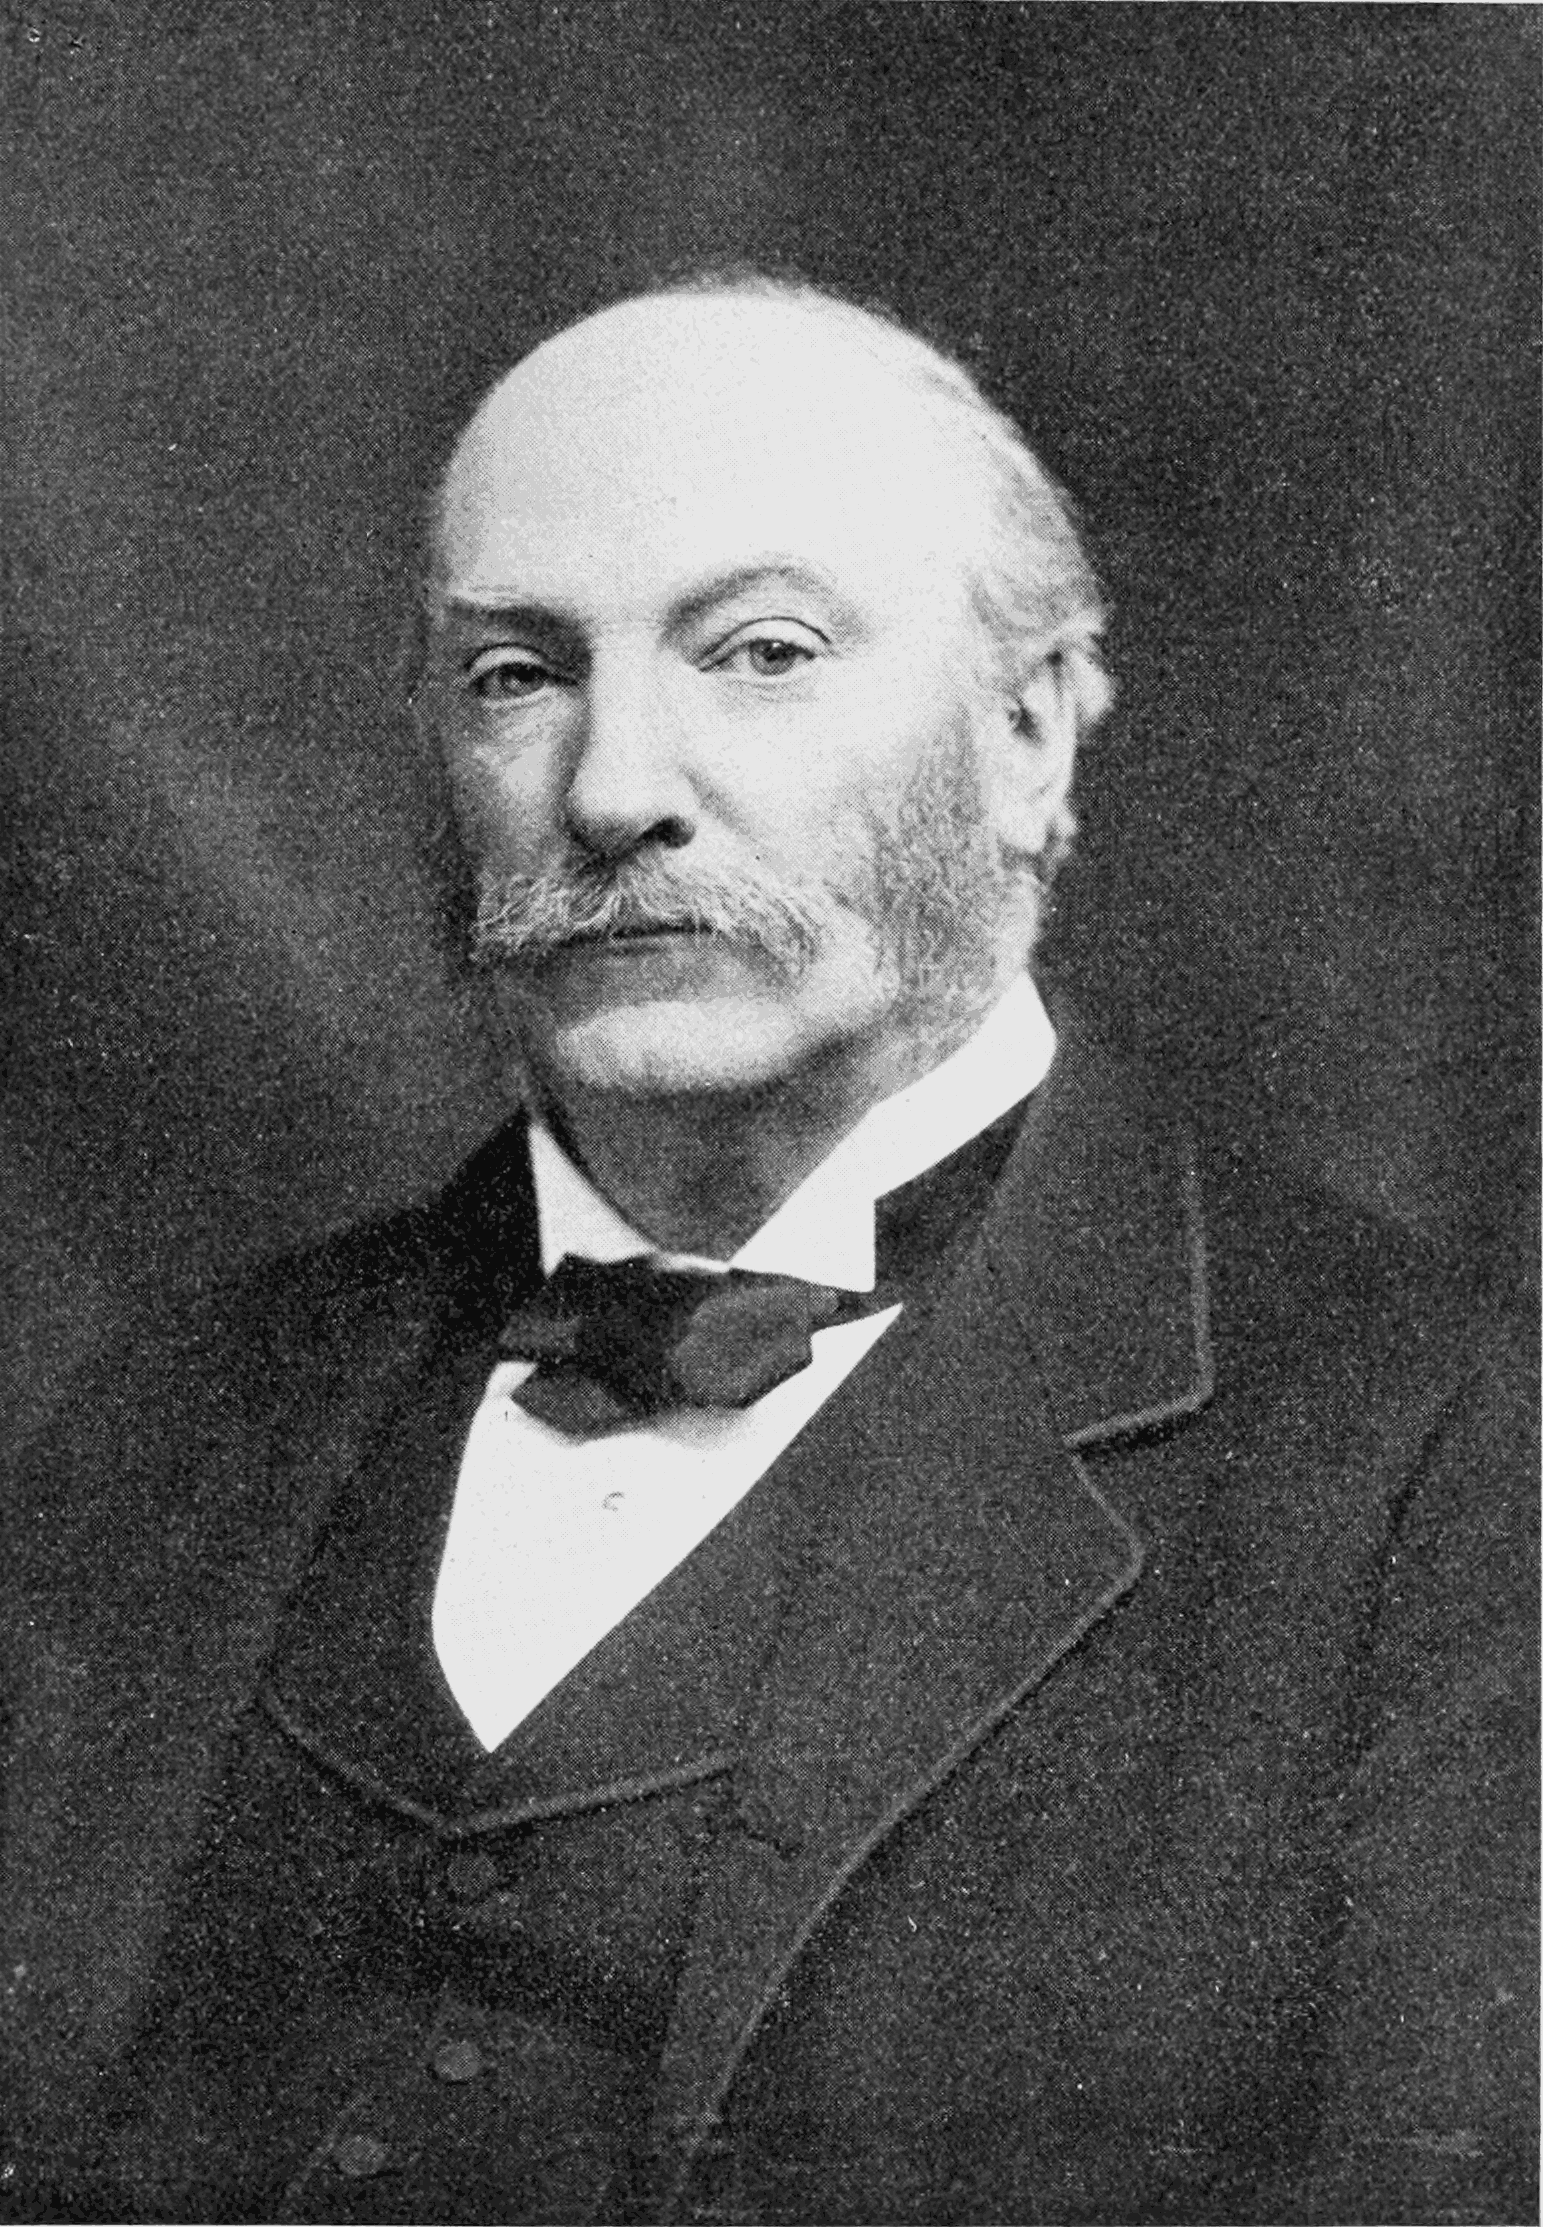
\includegraphics[height=.45\textheight]{img/reley.png}
      \caption{Дж. У. Рэлей}
    \end{subfigure}}
    \only<2->{\begin{subfigure}{.3\textwidth}
      \centering
      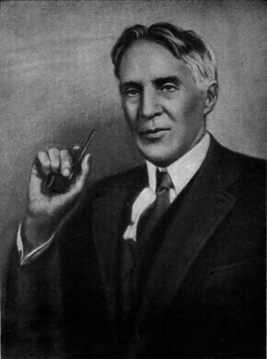
\includegraphics[height=.45\textheight]{img/wood.png}
      \caption{Р. У. Вуд}
    \end{subfigure}}
    \only<3->{\begin{subfigure}{.3\textwidth}
      \centering
      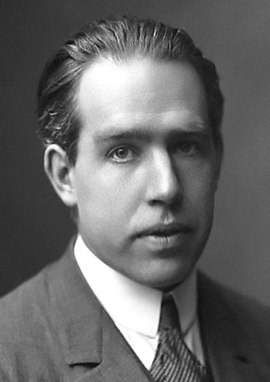
\includegraphics[height=.45\textheight]{img/bor.png}
      \caption{Н. Бор}
    \end{subfigure}}
  \end{figure}
\end{frame}

\begin{frame}
  \frametitle{Предыстория}
  \begin{itemize}
    \uncover<1->{\item Идея о том, что энергетические уровни ядер подобны
    электронным уровням атомов в работах Ч.~Д.~Эллиса (1920-е гг.).}
    \uncover<2->{\item Различие атомной и ядерной флоуресценции В.~Кун (1927 г.).}
    \uncover<3->{\item Первый успешный эксперимент на ядрах золота-198 (1950 г.).}
  \end{itemize}

  \begin{figure}[h]
    \captionsetup[subfigure]{labelformat=empty}
    \only<1->{\begin{subfigure}{\textwidth}
      \centering
      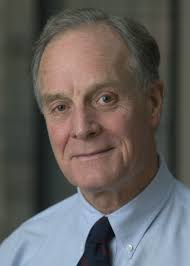
\includegraphics[height=.35\textheight]{img/ellis.png}
      \caption{Ч. Д. Эллис}
    \end{subfigure}}
  \end{figure}
\end{frame}

\begin{frame}
  \frametitle{Предыстория}
  \begin{itemize}
    \item Окончательно проблему решил Мёссбауэр
  \end{itemize}

  \begin{figure}[h]
    \centering
    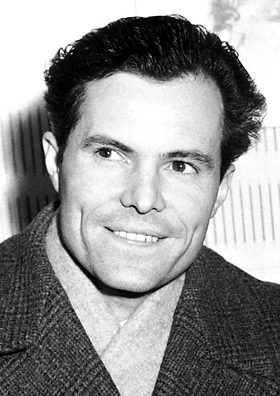
\includegraphics[height=.7\textheight]{img/messbauer.png}
  \end{figure}
\end{frame}

\end{document}
